\documentclass[runningheads,11pt]{llncs}

\usepackage[T1]{fontenc}
\usepackage{lmodern}
\usepackage{amsmath,amssymb}
\usepackage{booktabs}
\usepackage{array}
\usepackage{tikz}
\usetikzlibrary{arrows.meta,positioning,calc}
\usepackage{algorithm}
\usepackage[noend]{algpseudocode}
\usepackage[hidelinks]{hyperref}

\DeclareUrlCommand\file{\urlstyle{tt}}
\newcommand{\efxz}{\texorpdfstring{\mbox{EFX$_0$}}{EFX0}}
\newcommand{\st}{\mathrel{:}}
\newcommand{\DE}{\textup{DE}}
\algrenewcommand\algorithmiccomment[1]{\hfill$\triangleright$ #1}

\setlength{\emergencystretch}{1.5em}
\begin{document}

\title{\efxz{} Allocations with at Most Three Relevant Goods: A Short Proof}
\subtitle{Long version}
\titlerunning{\efxz{} with at Most Three Relevant Goods: A Short Proof (long version)}

\author{Evan Lin}
\authorrunning{E. Lin}
\institute{University of Illinois Urbana-Champaign}

\maketitle

\begin{abstract}
An allocation of indivisible goods is \efxz{} if no agent envies another agent's bundle after removing any single good from it, even a good that the envious agent values at zero. We give a short proof that every instance with nonnegative additive valuations in which each agent positively values at most three goods has a complete \efxz{} allocation in which all bundles but at most one have at most two goods. An algorithm we call Draft and Exchange (\DE{}) computes one in time $O(n(n+m))$. Agents that can leave with one good do so; the others draft at most one good each; then, until a free agent can take all the leftover goods (or every agent holds its pair), goods are traded along a chain or a ring of agents, each of which gets strictly better off. There are at most $4n$ trades. The key fact is that when no free agent can take the leftovers, the free agents have enough distinct obstacles to point at, and following these pointers closes a ring. The proof is machine-checked in Lean, together with the algorithm, its bound of $4n$ trades and its running time.
\keywords{Fair division \and Indivisible goods \and EFX \and Serial dictatorship \and Trading cycles}
\end{abstract}

%======================================================================
\section{Introduction}\label{sec:intro}

We allocate a set $M$ of $m$ indivisible goods to a set $N$ of $n\ge1$ agents. Agent $i$ has an \emph{additive valuation}: a value $v_i(g)\ge0$ for each good $g$, and $v_i(S)=\sum_{g\in S}v_i(g)$ for every set $S$ of goods. An \emph{allocation} $X$ gives every good to exactly one agent; $X_i$ is agent $i$'s \emph{bundle}. Every allocation in this paper is \emph{complete}: no good may be thrown away.

Envy-freeness can be impossible with indivisible goods (one good, two agents who value it). \emph{Envy-freeness up to any good} weakens it~\cite{AmanatidisBFV22}: the envy of $i$ for $X_j$ must disappear as soon as any single good is removed from $X_j$. Two versions differ in which goods may be removed:
\begin{align*}
\text{EFX:}&\quad v_i(X_i)\ge v_i(X_j\setminus\{h\})\quad\text{for all } i\ne j \text{ and } h\in X_j \text{ with } v_i(h)>0;\\
\text{\efxz{}:}&\quad v_i(X_i)\ge v_i(X_j\setminus\{h\})\quad\text{for all } i\ne j \text{ and } h\in X_j.
\end{align*}
\efxz{} implies EFX, and the two coincide when all values are positive. Whether every instance with additive valuations has a complete EFX allocation is a central open question of fair division~\cite{AmanatidisBFV22}. Under \efxz{}, if another agent's bundle contains a good that agent $i$ values at $0$, then $i$ must not envy that bundle at all, since removing that good does not lower its value to $i$.

\begin{example}[EFX, but not \efxz{}]\label{ex:efx-vs-efx0}
Two agents share goods $a$, $b$, $c$. Agent~1 values $a$, $b$, $c$ at $3$, $2$, $0$; agent~2 values only $c$, at $1$. The allocation $X_1=\{b\}$, $X_2=\{a,c\}$ is EFX: agent~1 may remove only $a$ from $X_2$, and $\{c\}$ is worth $0\le2$; agent~2 values $\{b\}$ at $0$. It is not \efxz{}: removing $c$ from $X_2$ leaves $\{a\}$, worth $3>2$ to agent~1. The allocation $X_1=\{a\}$, $X_2=\{b,c\}$ is \efxz{}.
\end{example}

\subsection{Results}\label{sec:results}

Write $R_i=\{g\in M\st v_i(g)>0\}$ for the goods agent $i$ values, its \emph{relevant} goods. If every agent values at most two goods, serial dictatorship works: the agents, in any order, each take a favourite remaining good, and the last agent takes everything left (\cite{MrdEfx}; Corollary~\ref{cor:k2} below). At three goods this breaks. An agent that values $a$, $b$, $c$ at $4$, $3$, $2$ may take $a$ and then see $b$ and $c$ end up in the last agent's bundle together with a third good; removing that third good leaves $b$ and $c$, worth $5>4$.

\begin{theorem}[existence]\label{thm:target}
Every instance with $n\ge1$ agents and nonnegative additive valuations in which every agent positively values at most three goods has a complete \efxz{} allocation.
\end{theorem}

\begin{theorem}[one large bundle]\label{thm:D}
Every such instance has a complete \efxz{} allocation in which all bundles but at most one have at most two goods.
\end{theorem}

\begin{theorem}[algorithm]\label{thm:algo}
Algorithm Draft and Exchange (\DE{}, Section~\ref{sec:algo}) computes such an allocation for every instance in which every agent positively values at most three goods, with at most $n$ peeling steps and at most $4n$ trades, in time $O(n(n+m))$. On real values, every decision of \DE{} compares two sums of at most two values of one agent.
\end{theorem}

\subsection{How the proof works}\label{sec:overview}

\emph{Peeling.} If an agent values its favourite remaining good at least as much as all its other remaining goods together, it takes that good and leaves; nobody envies a bundle of one good after removing it. When nobody can leave, every remaining agent values exactly three remaining goods $a\succ b\succ c$, with $v(a)<v(b)+v(c)$.

\emph{The draft.} The remaining agents, in turn, each take the best of their three goods still available, or nothing. Afterwards every good that an agent ranks above what it holds, a good it \emph{wants}, is held alone by another agent. We keep this property, \emph{validity}, throughout. The goods nobody took are \emph{leftover}.

\emph{Finishing.} To finish, one agent takes all the leftover goods. It must be \emph{free}: nobody may want its good. The only agents that could still envy its big bundle are its \emph{blockers}: agents holding their top good $a$ whose $b$ and $c$ would both be in it. Each blocker is fixed by moving one of these two goods, which is leftover, to another free agent, one good each. So a free agent can finish when its blockers' leftover goods are at most as many as the other free agents (Theorem~\ref{thm:sound}).

\emph{Improving.} If no free agent can finish, some agents can be made better off. If an agent holding its top finds its $b$ and $c$ both leftover, it takes them, and its top goes to an agent that wants it, and so on: a \emph{chain}. Otherwise every free agent failed to finish because it has at least as many blockers with distinct leftover goods as there are free agents, so each free agent can pick a blocker whose leftover good no other free agent picked. Now every agent points at someone who would gladly take its good: a free agent at its blocker, which completes its pair with that good and its leftover good, and any other agent at an agent that wants its good. Following the pointers closes a \emph{ring}, and passing the goods one step along it makes everyone on it better off (Theorem~\ref{thm:improve}). Scores only grow, so this ends, with a free agent that can finish or with every agent holding its pair. Section~\ref{sec:algo} ends with a small example, and Section~\ref{sec:example} has a larger one.

\paragraph{Status.} The proofs below are written proofs, and they are machine-checked in Lean~4, together with the algorithm, its bound of $4n$ trades, its running time, and its use on real values (Section~\ref{sec:evidence}). They were also checked by computer on millions of states. The reviews so far were by AI agents (Section~\ref{sec:evidence}); there has been no human peer review.

\paragraph{Related work.} For additive valuations, complete EFX allocations are known to exist only in special cases, among them: for three agents~\cite{ChaudhuryGM20} and for three types of agents~\cite{HVGNV25}; when $m\le n+3$~\cite{Mahara21}; for four agents and at most nine goods~\cite{AlkassarFM26}; when every good is valued by at most two agents~\cite{AfshinmehrAMMS26}, with special cases in~\cite{ChristodoulouFKS23,SgouritsaS25,KavianiSS24}; and for hypergraphs of girth at least four~\cite{LianeasSS26}. All of these use the all-goods form \efxz{}. For monotone valuations that are not additive, EFX allocations need not exist~\cite{AkramiMMSW26,MackenzieS26}. We restrict instead how many goods each agent values. For at most two goods per agent, serial dictatorship suffices and has been formalized in Lean~\cite{MrdEfx}. For at most four, Viswanathan and Mehta~\cite{ViswanathanM24} announce ordinary EFX allocations, with a polynomial-time algorithm and a proof sketch in an extended abstract; their algorithm gives the goods nobody values to an arbitrary agent, which is harmless for EFX but can break \efxz{} (Example~\ref{ex:efx-vs-efx0}). Since \efxz{} implies EFX, Theorem~\ref{thm:target} proves the case of three goods of their result in full. Table~\ref{tab:rw} in Appendix~\ref{app:rw} compares these results.

%======================================================================
\section{Peeling}\label{sec:peel}

Agents and goods are numbered, and ``index order'' and ``the first'' refer to these numbers. A good is \emph{alone} in an allocation if it is the only good of its bundle.

\begin{lemma}[peeling]\label{lem:peel}
Let $i\in N$ and $P\subseteq M$ with (i) $v_i(P)\ge v_i(M\setminus P)$ and (ii) $|P|\le1$. If the instance with agents $N\setminus\{i\}$ and goods $M\setminus P$ has an \efxz{} allocation $Z$, then $Z$ together with $X_i=P$ is an \efxz{} allocation of the whole instance.
\end{lemma}

\begin{proof}
Agent $i$ and a bundle $Z_j$: $v_i(Z_j\setminus\{h\})\le v_i(Z_j)\le v_i(M\setminus P)\le v_i(P)$. Agent $j\ne i$ and the bundle $P$: removing its only good leaves nothing. Agent $j\ne i$ and a bundle $Z_k$: this is a condition of $Z$. \qed
\end{proof}

\noindent \emph{Rule R1.} Let $G$ be the set of remaining goods, and $p$ agent $i$'s favourite good of $G$ (largest value, ties by index). If $v_i(p)=0$, then $i$ may leave with $P=\emptyset$. If $v_i(p)>0$ and $v_i(G\setminus\{p\})\le v_i(p)$, then $i$ may leave with $P=\{p\}$. Rule R1 applies, for instance, to every agent that values at most two remaining goods.

\begin{corollary}[two relevant goods]\label{cor:k2}
If $|R_i|\le2$ for every agent, then serial dictatorship, in any order of the agents, each taking a favourite remaining good (or nothing once no good is left), with the last agent taking all remaining goods, returns an \efxz{} allocation.
\end{corollary}

\begin{proof}
By induction on the number of agents. One agent faces no condition. Otherwise rule R1 applies to the first agent's choice, and Lemma~\ref{lem:peel} reduces to the smaller instance. \qed
\end{proof}

\noindent When $|R_i|=3$ we name agent $i$'s relevant goods $a_i$, $b_i$, $c_i$ so that $v_i(a_i)\ge v_i(b_i)\ge v_i(c_i)>0$, breaking ties by index. This gives a strict \emph{ranking} $a_i\succ_i b_i\succ_i c_i$, and $g\succ_i h$ implies $v_i(g)\ge v_i(h)$. Agent $i$ is \emph{strictly balanced} if $v_i(a_i)<v_i(b_i)+v_i(c_i)$.

\begin{lemma}[when nobody can leave]\label{lem:R1fail}
Let agent $i$ value at most three goods of the set $G$ of remaining goods, and suppose that rule R1 does not apply to $i$. Then $i$ values exactly three goods of $G$ and is strictly balanced with respect to them.
\end{lemma}

\begin{proof}
Rule R1 fails, so $v_i(p)>0$ and $v_i(G\setminus\{p\})>v_i(p)$. If $i$ valued at most two goods of $G$, then $v_i(G\setminus\{p\})$ would be the value of at most one good, at most $v_i(p)$. So $i$ values exactly three goods of $G$, $p$ is its top, and $v_i(b_i)+v_i(c_i)>v_i(a_i)$. \qed
\end{proof}

\noindent In Sections~\ref{sec:states}--\ref{sec:improve} we are in the \emph{core case}: every agent values exactly three goods and is strictly balanced. Goods that no agent values may exist.

%======================================================================
\section{States}\label{sec:states}

\begin{definition}[states and scores]\label{def:state}
A \emph{state} $Y$ gives each agent $i$ a \emph{holding} $Y_i$: nothing, $\{a_i\}$, $\{b_i\}$, $\{c_i\}$, or its \emph{pair} $\{b_i,c_i\}$, with the holdings pairwise disjoint. $U$ is the set of agents holding their pair. The goods held by nobody are \emph{leftover}; $J$ is the set of leftover goods. Agent $i$'s \emph{score} is $4$, $3$, $2$, $1$ or $0$ if it holds its pair, $a_i$, $b_i$, $c_i$ or nothing. Since $v_i(a_i)<v_i(b_i)+v_i(c_i)$, a higher score never means a lower value.
\end{definition}

\begin{definition}[wants, validity, free agents]\label{def:valid}
Let $Y$ be a state. An agent $i\notin U$ \emph{wants} a good $g\in R_i$ if it holds nothing, or holds a good $y$ with $g\succ_i y$. Agents in $U$ want nothing. $Y$ is \emph{valid} if every good that some agent wants is held alone: it is the whole holding of some agent. An agent $i\notin U$ is \emph{free} if it holds nothing or holds a good that nobody wants. $F$ is the set of free agents.
\end{definition}

\noindent No agent wants its own good, so in a valid state the holder of a wanted good is another agent, outside $U$ and not free. Leftover goods and the goods of pair holders are not wanted in a valid state. An agent outside $U\cup F$ holds a single good that some agent wants.

\begin{lemma}[the draft]\label{lem:draft}
Let the agents, in any order, each take the first of $a_i$, $b_i$, $c_i$ not yet taken, or nothing if all three are taken. The result is a valid state with $U=\emptyset$.
\end{lemma}

\begin{proof}
Each agent holds one of its goods or nothing, and no good is taken twice. If $i$ wants $g$, then $g$ was taken before $i$'s turn, by an earlier agent as its only good, and holdings never change during the draft. \qed
\end{proof}

\begin{lemma}[staying valid]\label{lem:stay}
Let $Y$ be valid, and $Y'$ a state in which every agent's score is at least its score in $Y$ and every good wanted in $Y$ is held alone. Then $Y'$ is valid.
\end{lemma}

\begin{proof}
Let $i$ want $g$ in $Y'$. If $i$ holds nothing in $Y'$, its score in $Y$ was $0$, so it held nothing in $Y$ and wanted $g$ there too. If $i$ holds a single good $y'$ in $Y'$, its score in $Y$ was below $4$, so in $Y$ it held nothing, or a good $y$ with $y'=y$ or $y'\succ_i y$; since $g\succ_i y'$, again $i$ wanted $g$ in $Y$. So $g$ is held alone in $Y'$. \qed
\end{proof}

%======================================================================
\section{Finishing}\label{sec:finish}

\begin{definition}[blockers, finishing]\label{def:finish}
Let $Y$ be a state and $o$ a free agent. A \emph{blocker} of $o$ is an agent $x\ne o$ that holds exactly its top, $Y_x=\{a_x\}$, and has $b_x,c_x\in J\cup Y_o$. Agent $o$ \emph{can finish} with a set $H\subseteq J$ if $|H|\le|F|-1$ and $H$ contains $b_x$ or $c_x$ for every blocker $x$ of $o$. Its \emph{completion} $X$ gives each good of $H$ to a different free agent other than $o$, gives $o$ the bundle $X_o=Y_o\cup(J\setminus H)$, and lets every other agent keep its holding (plus its good of $H$, if any).
\end{definition}

\noindent So a blocker of $o$ is an agent that would find both $b_x$ and $c_x$ in $o$'s bundle if $o$ took all the leftover goods; $H$ moves one of the two out of it. When every agent holds its pair, the completion with any agent $o$ gives $o$ the bundle $Y_o\cup J$ and lets the others keep their pairs.

\begin{theorem}[soundness]\label{thm:sound}
Let $Y$ be a valid state, and $X$ the completion with a free agent $o$ that can finish with a set $H$, or, if every agent holds its pair, with any agent $o$. Then $X$ is an \efxz{} allocation, and every bundle other than $X_o$ has at most two goods.
\end{theorem}

\begin{proof}
\emph{Sizes.} A free agent other than $o$ holds at most one good and receives at most one good of $H$; a pair holder holds two goods; every other agent keeps a single good.

\emph{Wanted goods stay alone.} Let $g$ be wanted, held alone by $j$. Then $j$ is not free, so $j\ne o$ and $j$ receives no good of $H$: $X_j=\{g\}$. Hence every good in a bundle of two or more goods is unwanted.

\emph{No envy.} Let $i\ne j$ and $h\in X_j$. We show $v_i(X_j\setminus\{h\})\le v_i(X_i)$, where $v_i(X_i)\ge v_i(Y_i)$. If $|X_j|\le1$, then $X_j\setminus\{h\}=\emptyset$. Let $|X_j|\ge2$, and $T=X_j\cap R_i$; it contains no good that $i$ wants and none of $i$'s holding.
\begin{itemize}
\item If $i$ holds its pair, then $T\subseteq\{a_i\}$, and $v_i(T)\le v_i(a_i)<v_i(b_i)+v_i(c_i)$.
\item If $i$ holds nothing, it wants all of $R_i$, so $T=\emptyset$.
\item If $Y_i=\{y\}$, every good of $T$ is ranked below $y$ and worth at most $v_i(y)$. If $|T|\le1$, then $v_i(X_j\setminus\{h\})\le v_i(T)\le v_i(y)$. If $|T|=2$, then $y=a_i$ and $T=\{b_i,c_i\}$. If $X_j=\{b_i,c_i\}$, removing $h$ leaves one good, worth at most $v_i(b_i)\le v_i(a_i)$. Otherwise $|X_j|\ge3$, so $j=o$ by the sizes, and $b_i,c_i\in X_o\subseteq Y_o\cup J$: $i$ is a blocker of $o$. Then $H$ contains $b_i$ or $c_i$, which went to an agent other than $o$, a contradiction. (When every agent holds its pair, only the first case occurs.) \qed
\end{itemize}
\end{proof}

%======================================================================
\section{Improving}\label{sec:improve}

\begin{definition}[rings]\label{def:ring}
Let $Y$ be a state. A \emph{ring} is a cycle $w_0\to w_1\to\dots\to w_{k-1}\to w_0$ of $k\ge2$ distinct agents outside $U$, each holding a single good $y_t=y_{w_t}$, such that each arrow $w_t\to w_{t+1}$ (indices modulo $k$) is
\begin{itemize}
\item a \emph{want arrow}: $w_{t+1}$ wants $y_t$; or
\item a \emph{pair arrow}: $w_t$ is free, $w_{t+1}$ is a blocker of $w_t$, and the pair of $w_{t+1}$ is $\{y_t,h_{t+1}\}$ with $h_{t+1}\in J$;
\end{itemize}
and the leftover goods $h_{t+1}$ of the pair arrows are pairwise distinct. \emph{Trading along the ring} gives each $w_{t+1}$ the good $y_t$, together with $h_{t+1}$ for a pair arrow, in place of its own good; agents off the ring keep their holdings.
\end{definition}

\noindent An arrow from a free agent is a pair arrow (nobody wants its good), and an arrow from any other agent is a want arrow.

\begin{lemma}[ring]\label{lem:ring}
Trading along a ring of a valid state gives a valid state in which every agent of the ring has a higher score and every other agent the same score.
\end{lemma}

\begin{proof}
\emph{A state.} Each good $y_t$ moves to $w_{t+1}$ only, and the goods $h_{t+1}$ are distinct leftover goods; agents off the ring keep goods that are neither. The new holdings are a single good of the receiver or its pair.
\emph{Scores.} Along a want arrow, $w_{t+1}$ receives a good it ranks above what it held. Along a pair arrow, $w_{t+1}$ goes from its top to its pair.
\emph{Wanted goods.} Let $g$ be wanted in $Y$, held alone by $j$. If $j$ is off the ring, it keeps $g$. If $j=w_t$, then $w_t$ is not free, so its arrow is a want arrow, and $w_{t+1}$ now holds $g$ alone. Lemma~\ref{lem:stay} gives validity. \qed
\end{proof}

\begin{lemma}[chain]\label{lem:chain}
Let $Y$ be valid, and $x$ an agent with $Y_x=\{a_x\}$ and $b_x,c_x\in J$. Let $j_0=x$, and as long as $j_t$ holds a good that some agent wants, let $j_{t+1}$ be the first such agent. If an agent repeats, the agents from its first occurrence on form a ring of want arrows. Otherwise the sequence stops at an agent $j_k$ ($k\ge0$) that holds nothing or a good nobody wants, and the following gives a valid state in which $x,j_1,\dots,j_k$ have higher scores and every other agent the same score: $x$ takes its pair; each $j_t$ with $1\le t\le k$ takes the good of $j_{t-1}$; the old good of $j_k$, if any, becomes leftover.
\end{lemma}

\begin{proof}
Agent $x$ holds its top and wants nothing, so $j_t\ne x$ for $t\ge1$. If $j_s=j_t$ with $1\le s<t$ is the first repeat, then $j_s,\dots,j_{t-1}$ are distinct agents outside $U$, each holding a good that the next one wants: a ring of want arrows ($t-s\ge2$, as no agent wants its own good). Otherwise: the goods $b_x$, $c_x$ were leftover, and each moved good moves one step, so this is a state. Agent $x$ goes from its top to its pair, and each $j_t$, $t\ge1$, receives a good it wants. A wanted good is not $b_x$ or $c_x$ (they are leftover); if its holder is off the path it stays, and if its holder is $j_t$, then $t<k$ (the good of $j_k$ is not wanted), and $j_{t+1}$ now holds it alone. Lemma~\ref{lem:stay} gives validity. \qed
\end{proof}

\noindent From now on, assume that no chain applies:

\smallskip
\noindent\textbf{(NC)} no agent $x$ with $Y_x=\{a_x\}$ has both $b_x$ and $c_x$ in $J$.
\smallskip

\begin{lemma}[the finishing test]\label{lem:test}
Let $Y$ be a state with (NC), and $o$ a free agent.
\begin{enumerate}
\item[(a)] If $o$ holds nothing, it has no blocker.
\item[(b)] If $x$ is a blocker of $o$, then $o$ holds a good $y_o$, and the pair of $x$ is $\{y_o,h_x\}$ for a leftover good $h_x$.
\item[(c)] Let $H_o$ be the set of the goods $h_x$ of the blockers $x$ of $o$. Then $o$ can finish if and only if $|H_o|\le|F|-1$, and then it can finish with $H_o$. In particular a free agent holding nothing can finish.
\end{enumerate}
\end{lemma}

\begin{proof}
Let $x$ be a blocker of $o$: $b_x,c_x\in J\cup Y_o$, and not both are in $J$, by (NC). So one of them is in $Y_o$, which proves (a), and, as $o$ holds at most one good, that good is $y_o$ and the other one, $h_x$, is leftover: (b). A set $H\subseteq J$ contains $b_x$ or $c_x$ if and only if it contains $h_x$; so the sets $H$ allowed by Definition~\ref{def:finish} are those with $H_o\subseteq H\subseteq J$ and $|H|\le|F|-1$, which exist if and only if $|H_o|\le|F|-1$. If $o$ holds nothing, $H_o=\emptyset$ and $|F|\ge1$. \qed
\end{proof}

\begin{theorem}[Improvement Lemma]\label{thm:improve}
Let $Y$ be a valid state in which not every agent holds its pair and no free agent can finish. Then a chain or a ring gives a valid state in which every agent has at least its score and some agent a higher one.
\end{theorem}

\begin{proof}
If (NC) fails, Lemma~\ref{lem:chain} applies. Assume (NC). By Lemma~\ref{lem:test}, every free agent $o$ holds a good and has $|H_o|\ge|F|$.

\emph{Distinct leftover goods.} List the free agents in index order, $o_1,\dots,o_f$. For $i=1,\dots,f$ in turn, pick $q_{o_i}\in H_{o_i}\setminus\{q_{o_1},\dots,q_{o_{i-1}}\}$, the first in index order; it exists because $|H_{o_i}|\ge f>i-1$. Let $x_{o_i}$ be the first blocker of $o_i$ with $h_{x_{o_i}}=q_{o_i}$.

\emph{Pointers.} For every agent $j\notin U$ let $\sigma(j)=x_j$ if $j$ is free, and otherwise let $\sigma(j)$ be the first agent that wants the good of $j$ (one exists, as $j\notin U\cup F$). In both cases $\sigma(j)\notin U$ and $\sigma(j)\ne j$.

\emph{The ring.} Start at the first agent outside $U$ and follow $\sigma$ until an agent repeats. The agents from its first occurrence on form a cycle $w_0\to\dots\to w_{k-1}\to w_0$ with $k\ge2$, each holding a single good (free agents by Lemma~\ref{lem:test}). The arrow from a free agent $w_t$ is a pair arrow, with $h_{t+1}=q_{w_t}$, by Lemma~\ref{lem:test}(b); these goods are distinct for distinct free agents. Every other arrow is a want arrow. So the cycle is a ring, and Lemma~\ref{lem:ring} applies. \qed
\end{proof}

\begin{corollary}[Pareto-optimal states]\label{cor:po}
In the core case, in every valid state that no valid state Pareto-dominates in scores, either every agent holds its pair or some free agent can finish. In particular every core instance has a complete \efxz{} allocation in which all bundles but one have at most two goods.
\end{corollary}

\begin{proof}
The first part is Theorem~\ref{thm:improve}. Valid states exist (Lemma~\ref{lem:draft}), there are finitely many, and one with the largest total score is Pareto-optimal; Theorem~\ref{thm:sound} finishes. \qed
\end{proof}

%======================================================================
\section{The Algorithm Draft and Exchange}\label{sec:algo}

Algorithm~\ref{alg:de} lists \DE{}. It receives the values $v_i(g)$; ties are broken by index as in Section~\ref{sec:peel}. Its loop runs on the core case left by peeling, with the notions of Sections~\ref{sec:states}--\ref{sec:improve}.

\begin{algorithm}[tb]
\caption{Draft and Exchange (\DE{})}\label{alg:de}
\begin{algorithmic}[1]
\Require agents $N$, goods $M$, nonnegative values $v_i(g)$, every agent with $|R_i|\le3$
\State $A\gets N$, $G\gets M$
\While{$|A|\ge2$ and rule R1 applies to some agent of $A$ with respect to $G$} \Comment{peeling}
  \State $i\gets$ the first such agent; $X_i\gets P_i$ (by rule R1); $A\gets A\setminus\{i\}$, $G\gets G\setminus P_i$
\EndWhile
\If{$|A|=1$} give $G$ to the agent of $A$ and \Return $X$ \EndIf
\For{$i\in A$ in index order} \Comment{the draft}
  \State $Y_i\gets$ the first of $\{a_i\},\{b_i\},\{c_i\}$ whose good is not taken, else nothing
\EndFor
\Loop
  \If{some $x$ with $Y_x=\{a_x\}$ has $b_x,c_x\in J$} \Comment{chain}
    \State apply the chain of the first such $x$ (Lemma~\ref{lem:chain})
  \ElsIf{every agent holds its pair} \Comment{finish}
    \State $o\gets$ the first agent; $H\gets\emptyset$; \textbf{break}
  \ElsIf{some free agent $o$ has $|H_o|\le|F|-1$} \Comment{finish}
    \State $o\gets$ the first such agent; $H\gets H_o$; \textbf{break}
  \Else \Comment{ring}
    \State trade along the ring of the proof of Theorem~\ref{thm:improve}
  \EndIf
\EndLoop
\State give the goods of $H$ to different free agents other than $o$, in index order
\State $X_o\gets Y_o\cup(J\setminus H)$; every other $i\in A$ keeps $Y_i$ (plus its good of $H$, if any)
\State \Return $X$
\end{algorithmic}
\end{algorithm}

\begin{theorem}[\DE{} is correct]\label{thm:de}
On every instance in which every agent values at most three goods, \DE{} returns a complete \efxz{} allocation in which all bundles but at most one have at most two goods. It peels at most $n$ agents and makes at most $4n$ trades.
\end{theorem}

\begin{proof}
\emph{Peeling.} Each round removes one agent, so there are at most $n$ rounds. Rule R1 for the agent $i$ peeled with $P_i$ is conditions (i) and (ii) of Lemma~\ref{lem:peel} on the instance left before it, so by induction from the last round down it suffices that \DE{} returns an \efxz{} allocation of the agents $A$ and goods $G$ left at the end. If $|A|=1$, the single agent faces no other bundle.

\emph{The core.} Let $|A|\ge2$. Rule R1 applies to no agent of $A$, so by Lemma~\ref{lem:R1fail} this is the core case. The draft gives a valid state (Lemma~\ref{lem:draft}). A chain or a ring gives a valid state in which nobody's score drops and some score rises (Lemmas~\ref{lem:chain} and~\ref{lem:ring}; the ring exists when it is used, by the proof of Theorem~\ref{thm:improve}). The total score is an integer between $0$ and $4|A|$, so there are at most $4|A|\le4n$ trades, and the loop stops. When it stops, $o$ can finish with $H$ (Lemma~\ref{lem:test}(c); the chain test failed, so (NC) holds), or every agent holds its pair; Theorem~\ref{thm:sound} gives an \efxz{} allocation in which only $X_o$ can have more than two goods. Peeled agents receive at most one good. \qed
\end{proof}

\paragraph{A small example.} Agents $z$, $x$, $o$, in index order, rank $g_5\succ g_0\succ g_1$, $g_0\succ g_1\succ g_2$ and $g_0\succ g_5\succ g_1$, with values $4$, $3$, $2$; nobody values $g_3$. Nobody is peeled. In the draft $z$ takes $g_5$, $x$ takes $g_0$, and $o$ takes $g_1$; the leftover goods are $g_2$, $g_3$. Agent $o$ wants $g_0$ and $g_5$, which are held alone: the state is valid, and $o$ is the only free agent. No chain applies. Agent $x$ is a blocker of $o$: if $o$ took $\{g_1,g_2,g_3\}$, $x$ would remove $g_3$ and see $g_1$ and $g_2$, worth $5>4$. So $H_o=\{g_2\}$, there is no other free agent to take $g_2$, and $o$ cannot finish. The pointers are $\sigma(o)=x$, a pair arrow ($x$'s pair is $o$'s good $g_1$ and the leftover $g_2$), and $\sigma(x)=\sigma(z)=o$, want arrows ($o$ wants $g_0$ and $g_5$). Following them from $z$ closes the ring $o\to x\to o$: $x$ takes $\{g_1,g_2\}$ and $o$ takes $g_0$. Now nobody wants anything, the free agents are $z$ and $o$, and $z$ has no blocker, so $z$ finishes: $X_z=\{g_5,g_3\}$, $X_x=\{g_1,g_2\}$, $X_o=\{g_0\}$, an \efxz{} allocation.

\paragraph{Running time.} An iteration of the loop needs the holder of each good, the goods each agent wants (at most three), the free agents, the blockers and their leftover goods, and a walk of at most $n$ steps. Once the chain test has failed, (NC) holds, and an agent holding only its top is a blocker of at most one free agent (Lemma~\ref{lem:test}(b)), so all blockers and the sets $H_o$ are found by one pass over the agents. With an array that records the holder of each good, an iteration takes $O(n+m)$ steps, and so does a round of peeling once the relevant goods of each agent are known. So \DE{} runs in $O(n(n+m))$ steps, reading the input included. This count is machine-checked in Lean, with one unit per elementary operation, array read and array write (Section~\ref{sec:evidence}).

\paragraph{Real values.} Every decision of \DE{} compares one value of an agent with another, or with the sum of two of its values (rule R1, the rankings), and the proofs use nothing else about the values. So Theorems~\ref{thm:target}--\ref{thm:algo} hold for nonnegative real values.

\begin{proof}[of Theorems~\ref{thm:target}, \ref{thm:D} and~\ref{thm:algo}]
Theorem~\ref{thm:de}, the running time and the remark on real values. \qed
\end{proof}

%======================================================================
\section{A Worked Example}\label{sec:example}

On this instance every improvement gives pairs to two agents at once, so a ring with a single pair arrow is not enough (Appendix~\ref{app:size}). Ten goods $g_0,\dots,g_9$ and six agents, in index order $x_1$, $x_1'$, $x_2$, $x_2'$, $o_1$, $o_2$, with values $4$, $3$, $2$ on their goods $a\succ b\succ c$ (any strictly balanced values with these rankings give the same run):
\begin{center}
\setlength{\tabcolsep}{6pt}\begin{tabular}{@{}llll@{}}
\toprule
agent & $a\succ b\succ c$ & after the draft & after the trade \\
\midrule
$x_1$ & $g_0\succ g_4\succ g_6$ & $\{g_0\}$ ($a$) & $\{g_4,g_6\}$ (pair) \\
$x_1'$ & $g_1\succ g_4\succ g_7$ & $\{g_1\}$ ($a$) & $\{g_1\}$ ($a$) \\
$x_2$ & $g_2\succ g_5\succ g_8$ & $\{g_2\}$ ($a$) & $\{g_5,g_8\}$ (pair) \\
$x_2'$ & $g_3\succ g_5\succ g_9$ & $\{g_3\}$ ($a$) & $\{g_3\}$ ($a$) \\
$o_1$ & $g_2\succ g_3\succ g_4$ & $\{g_4\}$ ($c$) & $\{g_2\}$ ($a$) \\
$o_2$ & $g_0\succ g_1\succ g_5$ & $\{g_5\}$ ($c$) & $\{g_0\}$ ($a$) \\
\bottomrule
\end{tabular}
\end{center}

\paragraph{The draft.} Nobody is peeled. The four $x$'s take their tops; $o_1$ finds $g_2$ and $g_3$ taken and takes $g_4$; $o_2$ takes $g_5$. Agent $o_1$ wants $g_2$ and $g_3$, $o_2$ wants $g_0$ and $g_1$, and the $x$'s want nothing; the four wanted goods are held alone. The leftover goods are $g_6,\dots,g_9$, and the free agents are $o_1$ and $o_2$. No chain applies: the $b$ of each $x$ is held by $o_1$ or $o_2$.

\paragraph{Nobody can finish.} The blockers of $o_1$ are $x_1$ (pair $\{g_4,g_6\}$) and $x_1'$ (pair $\{g_4,g_7\}$), so $H_{o_1}=\{g_6,g_7\}$; symmetrically $H_{o_2}=\{g_8,g_9\}$. Both have $|H_o|=2>|F|-1$. Concretely, if $o_1$ takes the leftovers, only $o_2$ can take one of $g_6$, $g_7$; with $H=\{g_6\}$, $X_{o_1}=\{g_4,g_7,g_8,g_9\}$, and $x_1'$, holding $g_1$ (worth $4$), values $X_{o_1}$ without $g_8$ at $3+2=5$. All ten candidate completions (finisher $o_1$ or $o_2$, with $H$ empty or one leftover good) fail the \efxz{} test.

\paragraph{No small trade helps.} A ring with no pair arrow would have to leave $o_1$ or $o_2$ by a want arrow, but nobody wants their goods. A ring with exactly one pair arrow, from $o_1$ say, would return to $o_1$ by want arrows; but $x_1$ and $x_1'$ have want arrows only to $o_2$, and the arrows from $o_2$ are pair arrows. In fact exactly four valid states Pareto-dominate the draft state, and each gives pairs to two agents.

\paragraph{The trade.} \DE{} picks $q_{o_1}=g_6$ (blocker $x_1$) and then $q_{o_2}=g_8$ (blocker $x_2$). So $\sigma(o_1)=x_1$, $\sigma(x_1)=o_2$ ($o_2$ wants $g_0$), $\sigma(o_2)=x_2$ and $\sigma(x_2)=o_1$ ($o_1$ wants $g_2$): the ring of Figure~\ref{fig:cycle}. Along it, $x_1$ takes $\{g_4,g_6\}$, $o_2$ takes $g_0$, $x_2$ takes $\{g_5,g_8\}$ and $o_1$ takes $g_2$. The total score rises from $14$ to $20$.

\begin{figure}[tb]
\centering
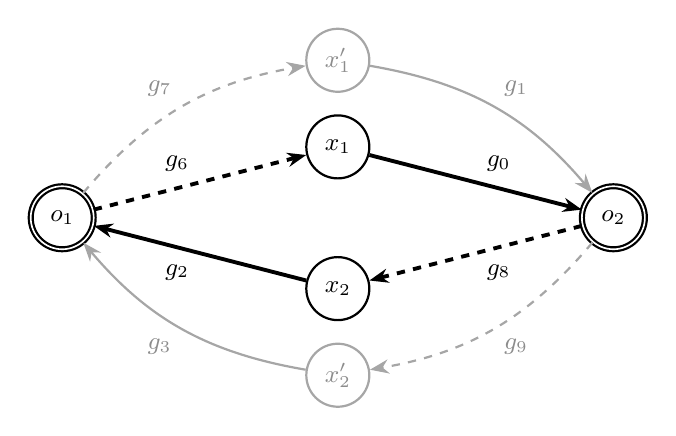
\begin{tikzpicture}[
  font=\small,
  ag/.style={draw, thick, circle, minimum size=8mm, inner sep=1pt},
  fr/.style={draw, thick, circle, double, minimum size=8mm, inner sep=1pt},
  need/.style={-{Stealth[length=2.4mm]}, thick},
  expo/.style={-{Stealth[length=2.4mm]}, thick, dashed},
  off/.style={draw=black!35, text=black!45}]
\node[fr] (o1) at (0,0) {$o_1$};
\node[fr] (o2) at (7,0) {$o_2$};
\node[ag] (x1) at (3.5,0.9) {$x_1$};
\node[ag, off] (x1p) at (3.5,2.0) {$x_1'$};
\node[ag] (x2) at (3.5,-0.9) {$x_2$};
\node[ag, off] (x2p) at (3.5,-2.0) {$x_2'$};
\draw[expo, line width=1.4pt] (o1) -- node[above left]{$g_6$} (x1);
\draw[need, line width=1.4pt] (x1) -- node[above right]{$g_0$} (o2);
\draw[expo, line width=1.4pt] (o2) -- node[below right]{$g_8$} (x2);
\draw[need, line width=1.4pt] (x2) -- node[below left]{$g_2$} (o1);
\draw[expo, black!35] (o1) to[bend left=20] node[above left, black!45]{$g_7$} (x1p);
\draw[need, black!35] (x1p) to[bend left=20] node[above right, black!45]{$g_1$} (o2);
\draw[expo, black!35] (o2) to[bend left=20] node[below right, black!45]{$g_9$} (x2p);
\draw[need, black!35] (x2p) to[bend left=20] node[below left, black!45]{$g_3$} (o1);
\end{tikzpicture}
\caption{The arrows of the draft state of Section~\ref{sec:example}. Double circles are the free agents. Dashed arrows are pair arrows, labelled by the blocker's leftover good; solid arrows are want arrows, labelled by the good that moves. The ring chosen by \DE{} is drawn in black. Every cycle of these arrows has four agents and two pair arrows.}\label{fig:cycle}
\end{figure}

\paragraph{Finishing.} Now nobody wants anything, the leftover goods are $g_7$ and $g_9$, and the free agents are $x_1'$, $x_2'$, $o_1$, $o_2$. No chain applies ($b$ of $x_1'$ is $g_4$, now held by $x_1$; similarly for the others). The first free agent, $x_1'$, has no blocker: no other agent holding its top has both $b$ and $c$ in $\{g_1,g_7,g_9\}$. So $x_1'$ finishes with $H=\emptyset$, and \DE{} returns
\begin{gather*}
X_{x_1}=\{g_4,g_6\},\quad X_{x_1'}=\{g_1,g_7,g_9\},\quad X_{x_2}=\{g_5,g_8\},\\
X_{x_2'}=\{g_3\},\quad X_{o_1}=\{g_2\},\quad X_{o_2}=\{g_0\}.
\end{gather*}
Directly: the only bundle of three goods, $X_{x_1'}$, is worth $3$ to $o_2$ (only $g_1$), which holds $g_0$, worth $4$, and $2$ to $x_2'$ (only $g_9$), which holds $g_3$, worth $4$; after removing one good, a bundle of two goods is worth at most $3$ to any other agent, and every agent holds at least $4$.

%======================================================================
\section{Verification}\label{sec:evidence}

\paragraph{Lean.} The proofs of Sections~\ref{sec:peel}--\ref{sec:algo} are machine-checked in core Lean~4 (\file{lean/EFX/K3DE*.lean} in~\cite{Repo}): no library beyond Lean's own, no unproved step, every declaration on Lean's three standard axioms, checked by the repository's \file{lean/check.sh}, which also replays the library in a fresh kernel. \DE{} is a Lean function, and the main theorem states that on every instance with natural-number values in which every agent positively values at most three goods it returns an \efxz{} allocation in which all bundles but at most one have at most two goods, after at most $n$ peeling rounds and $4n$ trades. The Lean files use earlier names for some notions: \emph{needs} for wants, \emph{exposed} for blocker, \emph{protecting good} for the leftover good $h_x$, \emph{need arcs} and \emph{exposure arcs} for want and pair arrows, \emph{valid absorber} for an agent that can finish, and \emph{pair chain} for a chain. One Lean lemma covers chains and rings (a chain is closed by an arrow from its last agent back to $x$).

Further files check the rest: Corollary~\ref{cor:k2}; DE on ordered values such as the nonnegative reals (it runs on natural-number values computed from the given ones with at most $n(m+12)$ comparisons, which answer every comparison of two subset sums of an agent as the given values do, so its output is \efxz{} for the given values); the facts of Section~\ref{sec:example} and Figure~\ref{fig:cycle} (by evaluation); Example~\ref{ex:efx-vs-efx0}; and the results of the appendices. The running time is checked on a counted program, proved to return exactly \DE{}'s output: at most $750(n+1)(n+m+1)$ units, reading the input included, with one unit per elementary operation, comparison, array read and array write, as in a random-access machine, arrays being used single-threaded. That the units match a machine is a property of the counted program, checked by reading it. The formal statements were written by AI agent sessions of the coding assistant that helped with this work (Claude Code) and compared with the text by independent AI sessions (\file{k3/simplify/po/referee/lean\_audit*.md} in~\cite{Repo}).

\paragraph{Tests.} The tests are evidence, not proof. Three implementations, each asserting every claim of a proof and checking outputs against the raw definition of \efxz{} with exact arithmetic, ran without failure on every profile with $n=2$ and $m\le6$, with $n=3$ and $m\le7$, and with $n=4$ and $m\le6$ (in part), on cores with $n=5,6$ and on random profiles with up to $9$ agents: about $1.7$ million valid states for the proof of Section~\ref{sec:improve}, about $15.5$ million for an independently found second proof (a walk instead of a choice of distinct leftover goods), and about $2.9$ million runs of a referee's implementation written from the text alone (\file{k3/simplify/po/} in~\cite{Repo}). The first and the referee's run \DE{}'s loop as stated here; the second tests the lemmas of Sections~\ref{sec:finish} and~\ref{sec:improve} on its own loop, which lets a free agent holding nothing finish first. The script \file{paper/k3-simple/examples/check\_examples.py}, written from this paper with the loop as stated here, recomputes every example and number of the paper and runs \DE{}, peeling included, on random instances with ties, unbalanced agents and goods nobody values.

%======================================================================
\section{Conclusion and Open Problems}\label{sec:concl}

Every instance in which each agent positively values at most three goods has a complete \efxz{} allocation with at most one bundle of more than two goods, and \DE{} computes one with at most $n$ peeling steps and $4n$ trades. The proof rests on one fact: if no free agent can take the leftover goods, then every agent can point at an agent that would gladly take its good, the free agents at blockers with distinct leftover goods, and the pointers close a ring along which everyone gains.

\emph{Open problems.} (1) \efxz{} with four relevant goods per agent (for ordinary EFX, see~\cite{ViswanathanM24}). With four goods an agent can hold one, two or three of them, and the order of holdings is not determined by the ranking alone, so the scores of Section~\ref{sec:states} have no direct analogue. (2) A better bound than $4n$ trades (at most $8$ were needed on random instances; from the draft, the rings of Appendix~\ref{app:size} of depth $4$ need up to $12$), or a draft that needs none. (3) The least size of the large bundle; Proposition~\ref{prop:neg}(b) shows that three goods do not always suffice.

\paragraph{Acknowledgments.} The proofs, code and the Lean formalizations were developed with the assistance of AI coding agents (Claude Code); this paper was also drafted with their assistance.

\bibliographystyle{splncs04}
\bibliography{refs}

\appendix

%======================================================================
\section{How Large Must a Ring Be?}\label{app:size}

Call a \emph{short move} a chain or a ring with at most one pair arrow. A natural simpler algorithm would use only short moves. The next proposition shows that the instance of Section~\ref{sec:example} is as small as possible in its number of agents among states where short moves are not enough.

\begin{proposition}[when short moves are not enough]\label{prop:short}
In the core case, let $Y$ be a valid state in which not every agent holds its pair, no free agent can finish, and no short move applies. Then $|F|\ge2$, $n\ge6$ and $m\ge8$; if $|F|\ge3$, then $n\ge9$ and $m\ge12$. The bounds $n=6$ and $m=8$ are attained.
\end{proposition}

\begin{proof}
No chain applies, so (NC) holds, and by Lemma~\ref{lem:test} every free agent $o$ holds a good and has at least $|H_o|\ge|F|$ blockers. The blockers of two different free agents $o,o'$ are different: a common blocker would have the pair $\{y_o,y_{o'}\}$, with no leftover good, against Lemma~\ref{lem:test}(b). There is no ring of want arrows, so a walk that repeatedly moves to an agent that wants the current agent's good never repeats an agent; it ends at an agent whose good nobody wants, or that holds nothing, which is free. Every agent holds a good: pair holders two, free agents one by Lemma~\ref{lem:test}, others a wanted good. Let $k=|F|$; $k\ge1$, because the walk from an agent outside $U$ ends at a free agent.

If $k=1$, let $F=\{o\}$ and $x$ a blocker of $o$. Then $x$ is not free, and its walk ends at $o$; with the pair arrow $o\to x$ this is a ring with one pair arrow, a short move. So $k\ge2$.

If $k=2$, let $F=\{o_1,o_2\}$. Agent $o_1$ has at least two blockers and only $o_2$ is another free agent, so some blocker $x$ of $o_1$ is not free. Its walk cannot end at $o_1$, as above, so it ends at $o_2$, entering it by a want arrow ($x\ne o_2$). So $o_2$ wants a good and does not hold its top: $o_2$ is not a blocker of $o_1$, and no blocker of $o_1$ is free. The same holds for $o_2$. So $n\ge2+2+2=6$, and $m\ge n+|J|\ge6+2=8$.

If $k\ge3$, the blockers of the $k$ free agents are at least $k^2$ different agents, at most $k$ of them free, so $n\ge|F|+(k^2-k)=k^2\ge9$, and $m\ge n+|J|\ge k^2+k\ge12$.

\emph{Attained.} The instance of Section~\ref{sec:example} has $n=6$ ($m=10$). For $m=8$: $o_1$ ranks $g_4\succ g_5\succ g_0$, $o_2$ ranks $g_6\succ g_7\succ g_1$, $x_1$ ranks $g_4\succ g_1\succ g_2$, $x_1'$ ranks $g_5\succ g_3\succ g_1$, $x_2$ ranks $g_6\succ g_0\succ g_2$, $x_2'$ ranks $g_7\succ g_3\succ g_0$, with $o_1$ holding $g_0$, $o_2$ holding $g_1$ and every $x$ its top. Then $J=\{g_2,g_3\}$, $F=\{o_1,o_2\}$, the blockers of $o_2$ are $x_1$, $x_1'$ (leftover goods $g_2$, $g_3$) and those of $o_1$ are $x_2$, $x_2'$ (leftover goods $g_2$, $g_3$); nobody can finish, and no short move applies. \qed
\end{proof}

\noindent In the second instance the distinct leftover goods matter: of the four cycles $o_2\to x\to o_1\to x'\to o_2$ with two pair arrows, two use the same leftover good twice, and trading along them would give it to two agents; the other two are rings.

\paragraph{No bounded number of pair arrows suffices.} For every $k\ge2$ and $d\ge1$ there are valid states with $k$ free agents $o_0,\dots,o_{k-1}$ in which $o_i$ wants the goods at the roots of a binary tree of depth $d$ of agents that want their children's goods, and the leaves of the tree of $o_{i+1}$ hold their tops and are blockers of $o_i$ (indices modulo $k$), with leftover goods that are distinct within each tree: one of its own per leaf, or the goods of a common pool of $k$, the leaves of each tree taking them in turn. Every cycle of want and pair arrows there has exactly $k$ pair arrows, and no free agent can finish if and only if $k\le2^d$, the number of leaves of a tree.

%======================================================================
\section{Limits of the Shape}\label{app:limits}

Could every instance have an \efxz{} allocation with all bundles of at most two goods, or with one bundle of exactly three? No. Write $\theta_i(B)$ for the largest value of $v_i(B\setminus\{h\})$ over $h\in B$ ($0$ if $B=\emptyset$): agent $i$ does not envy $X_j$ in the sense of \efxz{} if and only if $v_i(X_i)\ge\theta_i(X_j)$, and then $i$ is \emph{safe} if this holds for every $j\ne i$. By additivity, $\theta_i(B)=0$ if $|B|\le1$; $\theta_i(B)\le v_i(B\cap R_i)$, with equality if $B$ has a good outside $R_i$; and $\theta_i(\{g,h\})=\max(v_i(g),v_i(h))$.

\begin{lemma}[cases of safety]\label{lem:L5}
Let agent $i$ have $R_i=\{a,b,c\}$ with $v_i(a)>v_i(b)>v_i(c)>0$ and $v_i(a)<v_i(b)+v_i(c)$, and let $X$ be an allocation. Then $i$ is safe in $X$ if and only if one of the following holds:
\begin{description}
\item[(T)] $i$ holds $a$, and either $i$ also holds $b$ or $c$, or $b$ and $c$ are not together in a bundle of at least three goods;
\item[(BC)] $i$ holds $b$ and $c$;
\item[(B)] $i$ holds $b$, and $a$ is alone;
\item[(C)] $i$ holds $c$, and $a$ and $b$ are alone;
\item[(E)] $a$, $b$ and $c$ are all alone.
\end{description}
\end{lemma}

\begin{proof}
Write $a$, $b$, $c$ also for the values. The sums of subsets of $\{a,b,c\}$ are ordered as $0<c<b<a<b+c<a+c<a+b<a+b+c$. Let $S=X_i\cap R_i$.
\begin{itemize}
\item $S\supseteq\{a,b\}$ or $S\supseteq\{a,c\}$: every other bundle meets $R_i$ in at most one good, so its threat is at most $b<a+c$. Safe: (T).
\item $S=\{b,c\}$: every threat is at most $a<b+c$. Safe: (BC).
\item $S=\{a\}$: if $b$, $c$ are in different bundles, each threat is at most $b<a$; if $\{b,c\}$ is a bundle, its threat is $b<a$; if a bundle strictly contains $\{b,c\}$, it has a third good, outside $R_i$, and its threat is $b+c>a$. So: (T).
\item $S=\{b\}$: if $a$ is not alone, its bundle has threat at least $a>b$; if $a$ is alone, every threat is at most $c<b$. So: (B).
\item $S=\{c\}$: as before $a$ must be alone, and if $b$ is not alone its bundle has threat at least $b>c$. So: (C).
\item $S=\emptyset$: a bundle with a good of $R_i$ and at least two goods has a positive threat. So: (E).
\end{itemize}
Conversely, each of (T), (BC), (B), (C), (E) describes safe situations above: (T) is the first and third items; (BC) is $S=\{b,c\}$ or $S=\{a,b,c\}$; (B) forces $a\notin S$, so $S=\{b\}$ with $a$ alone, or $S=\{b,c\}$; (C) forces $S=\{c\}$ with $a$ and $b$ alone; and (E) means that $S$ is empty or a single alone good, which is (T), (B) or (C). \qed
\end{proof}

\begin{proposition}[limits of the shape]\label{prop:neg}
Take values with $v_i(a_i)>v_i(b_i)>v_i(c_i)>0$ and $v_i(a_i)<v_i(b_i)+v_i(c_i)$ for every agent.
\begin{enumerate}
\item[(a)] Let agents $0$, $1$, $2$ rank $g_0\succ g_1\succ p_i$, where $p_i$ is valued only by agent $i$. No \efxz{} allocation has all bundles of at most two goods, and $\{g_0\},\{g_1\},\{p_0,p_1,p_2\}$, to the three agents in any order, is \efxz{}.
\item[(b)] Let agents $0$, $1$, $2$, $3$ rank $g_0\succ g_2\succ p_0$, $g_0\succ g_2\succ p_1$, $g_1\succ g_2\succ p_2$ and $g_1\succ g_2\succ p_3$, with $p_i$ valued only by agent $i$. Every \efxz{} allocation has bundle sizes $4,1,1,1$, and one exists.
\end{enumerate}
\end{proposition}

\begin{proof}
(a) Five goods in three bundles of at most two goods have sizes $2,2,1$, so exactly one good is alone. Two agents do not hold their top $g_0$: case (T) fails for them, and (C) and (E) need two or three alone goods. So both are in case (BC) or (B), and both hold $g_1$, which is impossible. In $\{g_0\},\{g_1\},\{p_0,p_1,p_2\}$ the three agents are in cases (T), (B) and (C).

(b) Each of the tops $g_0$, $g_1$ has an agent ranking it first that does not hold it, a \emph{loser}; the two losers differ. A loser is safe only by (BC) or (B), which need it to hold $g_2$, or by (C) or (E), which need $g_2$ alone. The two losers cannot both hold $g_2$, so $g_2$ is alone, and nobody is in case (BC). A loser holding $\{g_2\}$ needs its top alone; a loser not holding $g_2$ needs its top and $g_2$ alone. So $g_0$, $g_1$, $g_2$ are alone, held by three agents, and the fourth bundle is $\{p_0,p_1,p_2,p_3\}$. Such an allocation exists: $g_0$ to agent~$0$, $g_1$ to agent~$2$, $g_2$ to agent~$1$, the four goods $p_i$ to agent~$3$ (cases T, B, T, C). \qed
\end{proof}

\noindent In (a) every agent values exactly three goods and is strictly balanced, so the one large bundle of Theorem~\ref{thm:D} cannot be avoided; by (b), its size cannot be bounded by three.

%======================================================================
\section{Related Work in a Table}\label{app:rw}

\begin{table}[htbp]
\caption{Existence results for complete allocations under restrictions. \emph{Version cited}: the published version where one exists, else arXiv. $^a$Goods nobody values go to an arbitrary agent. $^b$Includes additive. $^c$Extended abstract with a proof sketch. $^d$An AAMAS 2025 extended abstract has the degree and girth conditions. $^e$Accepted at EC 2026.}\label{tab:rw}
\centering\scriptsize
\setlength{\tabcolsep}{3pt}\begin{tabular}{@{}>{\raggedright\arraybackslash}p{0.08\textwidth}>{\raggedright\arraybackslash}p{0.24\textwidth}>{\raggedright\arraybackslash}p{0.08\textwidth}>{\raggedright\arraybackslash}p{0.11\textwidth}>{\raggedright\arraybackslash}p{0.14\textwidth}>{\raggedright\arraybackslash}p{0.13\textwidth}>{\raggedright\arraybackslash}p{0.11\textwidth}@{}}
\toprule
Result & Restriction (agents, goods, who values what) & Notion & Complete & Valuations & Algorithm & Version cited \\
\midrule
\cite{ChaudhuryGM20} & $n=3$ & \efxz{} & yes & additive & pseudo-polynomial & JACM 2024 \\
\cite{HVGNV25} & at most three distinct valuations & \efxz{} & yes & additive & no bound stated & EC 2025 \\
\cite{Mahara21} & $m\le n+3$ & \efxz{} & yes & monotone & none stated & MOR 2024 \\
\cite{AlkassarFM26} & $n=4$, $m\le9$ & \efxz{} & yes & additive & none stated & arXiv \\
\cite{ChristodoulouFKS23} & graphs: at most two valuers per good, two agents share at most one good & \efxz{} & yes & monotone & polynomial time & MOR 2026 (EC 2023) \\
\cite{AfshinmehrAMMS26} & multigraphs: at most two valuers per good & \efxz{} & yes & cancelable$^b$ & polynomial time & arXiv$^e$ \\
\cite{SgouritsaS25} & multigraphs: bipartite, or at most $\lceil n/4\rceil-1$ neighbours per agent, or girth at least six (non-parallel edges) & \efxz{} & yes & monotone & not efficient (stated) & arXiv$^d$ \\
\cite{KavianiSS24} & at most two valuers per good, $v_i(g)\in\{0,v_g\}$ & \efxz{} & yes & restricted additive & no time bound stated & WINE 2024 \\
\cite{LianeasSS26} & hypergraphs of girth at least four (a good joins its valuers) & \efxz{} & yes & monotone & polynomial time & AAAI 2026 \\
\cite{ViswanathanM24} & at most four relevant goods per agent & EFX & yes$^a$ & additive & polynomial time, announced & AAMAS 2024$^c$ \\
\cite{MrdEfx} & at most two relevant goods per agent & \efxz{} & yes & additive; monotone & serial dictatorship; Lean-checked & GitHub, v1.2.0 \\
this paper & at most three relevant goods per agent; any number of valuers per good & \efxz{} & yes & additive & polynomial time, at most $4n$ trades & this paper \\
\bottomrule
\end{tabular}
\end{table}

\end{document}
